\subsection{Модел с обобщена мрежа на производството на тежки нефтопродукти в нефтопреработвателна рафинерия}

\paragraph{Декларация за принос (съвместна публикация).}
\mbox{}\\
Разделът обобщава и интегрира резултати от съвместната публикация~\cite{Stratiev2023_2}.
Личният принос на докторанта се състои в: (i) съвместно конструиране на ОМ по описанието на процеса;
(ii) изпълнение на пълната симулация в \textit{OnlineGN} с цел верификация на модела и обработка на получените резултати;
(iii) изготвяне на илюстративния материал (всички фигури от симулациите) и описание на симулационния ход в текста.
%here i put new page command
\newpage
Тук се разглежда ОМ модел на производството на тежки нефтопродукти в нефтопреработвателна рафинерия и неговата симулация чрез \textit{OnlineGN}.
Изграждането на модела е описано подробно в гореспоменатата публикация~\cite{Stratiev2023_2}.

\subsubsection{Увод в обобщеномрежовите модели за нефтопродукти в нефтопреработвателна рафинерия}


\hspace*{2.5em}В предходния раздел бе показано, че паралелно протичащите производствени процеси в нефтопреработвателна рафинерия могат да бъдат моделирани и симулирани посредством ОМ~\cite{Z1}. В настоящата глава фокусът се премества към частта от технологичната схема, свързана с преработката на тежките остатъчни фракции и производството на тежки нефтени продукти, която до момента не е била представена с ОМ.

Тежкият нефт представлява остатъчната нефтена фракция, която остава след атмосферна дестилация на суровия нефт~\cite{96}. Той съдържа компоненти с температура на кипене над 360~$^\circ$C и относителна плътност над 0.933 (\textit{API} < 20)~\cite{97}. В нефтопреработвателна рафинерия тази фракция се подлага на допълнителна обработка с цел извличане на допълнителни количества леки нефтени продукти и производство на тежки нефтени продукти като горивни масла, корабни горива и битум за пътни настилки~\cite{98}.

Процесите в технологичната верига за обработка на тежък нефт са обект на моделиране и симулация с цел по-добро разбиране на поведението на инсталациите и определяне на стойностите на оперативните променливи, които осигуряват оптимална работа от икономическа, енергоспестяваща и екологична гледна точка~\cite{103,104}. Например в ~\cite{103} се симулира работата на вакуумната дестилация на атмосферни остатъци чрез \textit{Chemcad 5.1} с цел намаляване на енергийното потребление, а в ~\cite{104} се моделира индустриален реактор със суспензионна фаза (\textit{SPR}) за хидрокрекинг на вакуумни остатъци, използвайки различни кинетични модели.

Посочените и сходни разработки са частични модели на отделни процеси за обработка на тежък нефт и често служат като вход към планови/оптимизационни модели на ниво рафинерия. В настоящата глава паралелният характер на технологичната верига се разглежда чрез ОМ модел, който позволява едновременно описание на структурните връзки и логиката на протичане на процесите, както и симулация при зададени сценарии.

Целта на настоящото изследване е да се анализира процесът по производство на различни видове тежко гориво и битум за пътни настилки в рамките на нефтопреработвателна рафинерия, да се моделира с помощта на ОМ и моделът да бъде симулиран чрез \textit{OnlineGN}.
\subsubsection{Схема на преработка за производство на различни видове тежко гориво и битум за пътни настилки в нефтопреработвателна рафинерия, моделирана чрез обобщени мрежи}

\hspace*{2.5em}Горивата, използвани основно като гориво за товарни кораби, са известни и като морски горива. Световното търсене на морски горива се оценява на около 640 000 тона на ден, което подчертава значението на този вид гориво за световната икономика~\cite{123}. В изследваната рафинерия (ЛУКОЙЛ Нефтохим Бургас, ЛНБ) се получават три вида гориво с различно съдържание на сяра: гориво с масово съдържание на сяра $\leq$ 0.5 \% (\textit{Fuel oil} 0.5\%~\textit{S}); гориво със съдържание на сяра $\leq$ 1.0\% (\textit{Fuel oil} 1.0\%~\textit{S}); и гориво със съдържание на сяра $\leq$ 2.5\% (\textit{Fuel oil} 2.5\%~\textit{S}), както е показано на \textbf{Фигура~\ref{fig1}}.

Спецификациите на трите вида гориво, произвеждани в рафинерията ЛНБ са представени подробно в статия  ~\cite{Stratiev2023_2}. Горивата, произведени в рафинерията ЛНБ, се предлагат на пазара в съответствие с приложимите изисквания, представени в~\cite{Stratiev2023_2}.

\begin{figure}[H]
  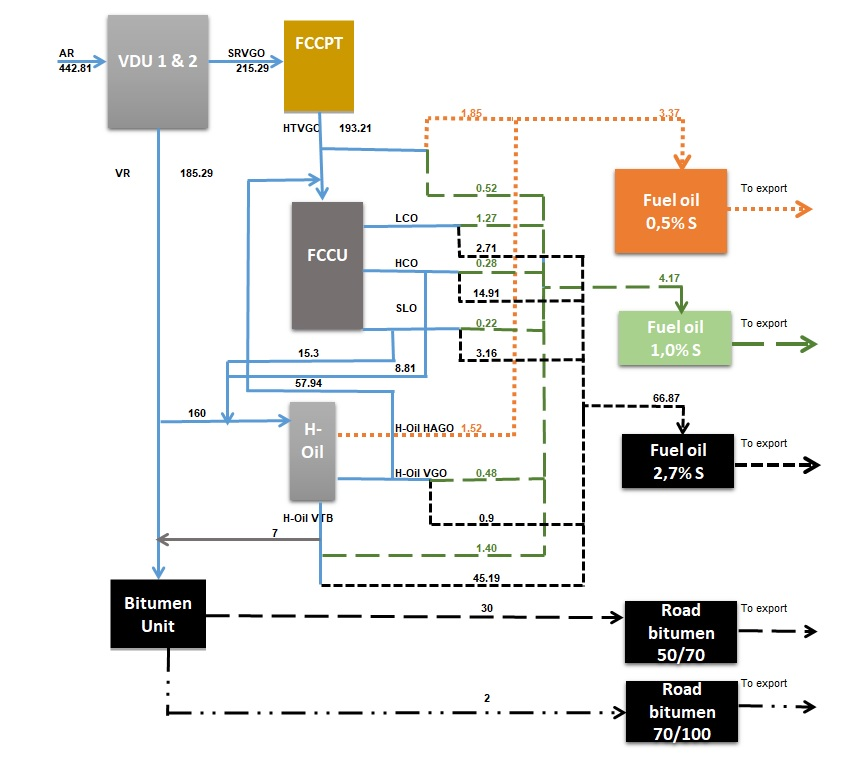
\includegraphics[scale=0.65]{4. applications/heavyOilProducts/images/Figure_1.jpg}%
  \caption{Схема на преработка
за производство на различни видове тежко гориво и битум за пътни настилки в нефтопреработвателна рафинерия, която ще бъде моделирана чрез обобщени мрежи (Числата в диаграмата съответстват на количеството потоци от тежък нефт в размер на t/h. Използвани са различни цветове за разграничаване на трите вида произведени горива: оранжев -- за гориво с 0.5\%~S, зелен -- за гориво с 1.0\%~S и черен -- за гориво с 2.5\%~S).}\label{fig1}
\end{figure}


\textbf{Фигура~\ref{fig1}} показва, че производството на битум за пътни настилки се осъществява в битумната инсталация (\textit{BU}), където смес от директен вакуумен остатък и \textit{H-Oil VTB} се подлага на окисление за получаване на два класа пътен битум: 50/70 и 70/100.

Подробности относно производството на пътен битум от директен вакуумен остатък (\textit{VR}) и \textit{H-Oil VTB} могат да се намерят в скорошно изследване~\cite{124}. Както се вижда и от \textbf{Фигура~\ref{fig1}}, вакуумният остатък (\textit{VR}) и вакуумният газьол от пряк добив (\textit{SRVGO}), използвани за производство на компонентите за горивата, както и на пътния битум, се получават в инсталациите за вакуумна дестилация (\textit{VDU-1} и \textit{VDU-2}), където атмосферният остатък, получен от инсталациите за първична дестилация на суров нефт (\textit{CDU}), се фракционира. Подробности относно работата на инсталациите за вакуумна дестилация са представени в~\cite{103}.

\subsubsection{Резултати от моделирането на производството на тежки нефтени продукти в нефтопреработвателна рафинерия с помощта на обобщени мрежи}

\hspace*{2.5em}ОМ моделът, показан на \textbf{Фигура~\ref{fig2}} съдържа 8 прехода, 35 позиции и 8 типа ядра. Значението на преходите е следното:

\begin{itemize}
	\item[$\bullet$] \textbf{\textit{VDU}} —  инсталация за вакуумна дестилация на мазута
	\item[$\bullet$] \textbf{\textit{FCCPT}} — инсталация за хидроочистване на суровината за каталитичен крекинг
	\item[$\bullet$] \textbf{\textit{H-Oil}} —  инсталация за хидрокрекинг на гудрон (\textit{H-Oil})
	\item[$\bullet$] \textbf{\textit{FCCU}} — инсталация за каталитичен крекинг на вакуумен газьол
	\item[$\bullet$] \textbf{\textit{BU}} —  инсталация за производство на пътни битуми
	\item[$\bullet$] \textbf{0.5 \textit{S}} — котелно гориво със съдържание на сяра не по-високо от 0.5~мас.\,\% \textit{S}
	\item[$\bullet$] \textbf{1.0 \textit{S}} — котелно гориво със съдържание на сяра не по-високо от 1.0~мас.\,\% \textit{S}
	\item[$\bullet$] \textbf{2.5 \textit{S}} — котелно гориво, съдържащо максимум 2.5~мас.\,\% \textit{S}
\end{itemize}



В началния момент от функционирането на ОМ ядрото $\alpha_0$ се намира в позиция $l_1$ с начална характеристика:
$$„\mbox{Атмосферен остатък (\textit{AR}), начално количество}“;$$
ядрото $\beta_0$ се намира в позиция $l_9$ с начална характеристика:
$$„\mbox{Пряко дестилатен вакуумен газьол (\textit{SRVGO}), начално количество}“;$$
ядрото $\gamma_0$ се намира в позиция $l_{17}$ с начална характеристика:
$$„\mbox{\textls[-15]{Смес от пряко дестилатен вакуумен остатък (\textit{SRVR}), \textit{FCC HCO} и \textit{FCC SLO}, начално количество}}“;$$
ядрото $\delta_0$ се намира в позиция $l_{26}$ с начална характеристика:
$$„\mbox{Смес от вакуумни газьоли, състояща се от \textit{SRVGO} и \textit{H-Oil VGO}, начално количество}“;$$
ядрото $\epsilon_0$ се намира в позиция $l_{29}$ с начална характеристика:
$$„\mbox{Смес от \textit{SRVR} и хидрокрекиран вакуумен остатък, начално количество}“;$$
ядрото $\zeta_0$ се намира в позиция $l_{31}$ с начална характеристика:
$$„\mbox{Гориво мазут с максимално съдържание на сяра 0{,}5~мас.~\%, начално количество}“;$$
ядрото $\eta_0$ се намира в позиция $l_{33}$ с начална характеристика:
$$„\mbox{Гориво мазут с максимално съдържание на сяра 1{,}0~мас.~\%, начално количество}“;$$
ядрото $\theta_0$ се намира в позиция $l_{35}$ с начална характеристика:
$$„\mbox{Гориво мазут с максимално съдържание на сяра 2{,}5~мас.~\%, начално количество}“;$$

Във всеки следващ момент от времето, в позиция $l_1$ постъпват ядра $\alpha_1, \alpha_2, ...$ с начални характеристики:
$$„\mbox{\textit{AR}, текущо постъпващо количество}“.$$

\begin{figure}[H]
		\tiny
	\newcommand{\mytriangle}{\Large $\bigtriangledown$}
	%\begin{center}
%		\begin{center}
		\setlength{\unitlength}{8.5pt} %10pt=4mm
		\linethickness{0.4pt}
		\begin{picture}(37, 71)
			%%% Transitions
			\put(3.0,71.0){\makebox(0,0)[cc]{$VDU$}}
			\put(3.0,69.0){\makebox(0,0)[bb]{\mytriangle}}
			\put(3.0,69.0){\line(0,-1){39}}
			\put(34.0,71){\makebox(0,0)[cc]{$BU$}}
			\put(34.0,69.0){\makebox(0,0)[bb]{\mytriangle}}
			\put(34.0,69.0){\line(0,-1){7}}
			\put(20.0,65.0){\makebox(0,0)[cc]{$H-Oil$}}
			\put(20.0,63.0){\makebox(0,0)[bb]{\mytriangle}}
			\put(20.0,63.0){\line(0,-1){17}}
			\put(34.0,57){\makebox(0,0)[cc]{$0.5\% S$}}
			\put(34.0,55.0){\makebox(0,0)[bb]{\mytriangle}}
			\put(34.0,55.0){\line(0,-1){7}}
			\put(20.0,39.0){\makebox(0,0)[cc]{$FCCU$}}
			\put(20.0,37.0){\makebox(0,0)[bb]{\mytriangle}}
			\put(20.0,37.0){\line(0,-1){19}}
			\put(34.0,39.0){\makebox(0,0)[cc]{$1.0\% S$}}
			\put(34.0,37.0){\makebox(0,0)[bb]{\mytriangle}}
			\put(34.0,37.0){\line(0,-1){15}}
			\put(10.0,37.0){\makebox(0,0)[cc]{$FCCPT$}}
			\put(10.0,35.0){\makebox(0,0)[bb]{\mytriangle}}
			\put(10.0,35.0){\line(0,-1){11}}
			\put(34.0,17.0){\makebox(0,0)[cc]{$2.5\% S$}}
			\put(34.0,15.0){\makebox(0,0)[bb]{\mytriangle}}
			\put(34.0,15.0){\line(0,-1){13}}
			%%% Input places
			\put(1.5,68.5){\makebox(0,0)[cc]{$l_{1}$}}
			\put(1.5,67.5){\circle{1.0}}
			\put(2.0,67.5){\vector(1,0){1.0}}
			%%% Output places
			\put(4.5,68.5){\makebox(0,0)[cc]{$l_{2}$}}
			\put(3.0,67.5){\vector(1,0){1.0}}
			\put(4.5,67.5){\circle{1.0}}
			\put(35.5,68.5){\makebox(0,0)[cc]{$l_{27}$}}
			\put(34.0,67.5){\vector(1,0){1.0}}
			\put(35.5,67.5){\circle{1.0}}
			\put(35.5,66.5){\makebox(0,0)[cc]{$l_{28}$}}
			\put(34.0,65.5){\vector(1,0){1.0}}
			\put(35.5,65.5){\circle{1.0}}
			\put(35.5,64.5){\makebox(0,0)[cc]{$l_{29}$}}
			\put(34.0,63.5){\vector(1,0){1.0}}
			\put(35.5,63.5){\circle{1.0}}
			\put(4.5,62.5){\makebox(0,0)[cc]{$l_{3}$}}
			\put(3.0,61.5){\vector(1,0){1.0}}
			\put(4.5,61.5){\circle{1.0}}
			\put(21.5,62.5){\makebox(0,0)[cc]{$l_{10}$}}
			\put(20.0,61.5){\vector(1,0){1.0}}
			\put(21.5,61.5){\circle{1.0}}
			\put(21.5,60.5){\makebox(0,0)[cc]{$l_{11}$}}
			\put(20.0,59.5){\vector(1,0){1.0}}
			\put(21.5,59.5){\circle{1.0}}
			\put(21.5,58.5){\makebox(0,0)[cc]{$l_{12}$}}
			\put(20.0,57.5){\vector(1,0){1.0}}
			\put(21.5,57.5){\circle{1.0}}
			\put(21.5,56.5){\makebox(0,0)[cc]{$l_{13}$}}
			\put(20.0,55.5){\vector(1,0){1.0}}
			\put(21.5,55.5){\circle{1.0}}
			\put(21.5,54.5){\makebox(0,0)[cc]{$l_{14}$}}
			\put(20.0,53.5){\vector(1,0){1.0}}
			\put(21.5,53.5){\circle{1.0}}
			\put(35.5,54.5){\makebox(0,0)[cc]{$l_{30}$}}
			\put(34.0,53.5){\vector(1,0){1.0}}
			\put(35.5,53.5){\circle{1.0}}
			\put(21.5,52.5){\makebox(0,0)[cc]{$l_{15}$}}
			\put(20.0,51.5){\vector(1,0){1.0}}
			\put(21.5,51.5){\circle{1.0}}
			\put(21.5,50.5){\makebox(0,0)[cc]{$l_{16}$}}
			\put(20.0,49.5){\vector(1,0){1.0}}
			\put(21.5,49.5){\circle{1.0}}
			\put(35.5,50.5){\makebox(0,0)[cc]{$l_{31}$}}
			\put(34.0,49.5){\vector(1,0){1.0}}
			\put(35.5,49.5){\circle{1.0}}
			\put(21.5,48.5){\makebox(0,0)[cc]{$l_{17}$}}
			\put(20.0,47.5){\vector(1,0){1.0}}
			\put(21.5,47.5){\circle{1.0}}
			\put(21.5,36.5){\makebox(0,0)[cc]{$l_{18}$}}
			\put(20.0,35.5){\vector(1,0){1.0}}
			\put(21.5,35.5){\circle{1.0}}
			\put(4.5,34.5){\makebox(0,0)[cc]{$l_{4}$}}
			\put(3.0,33.5){\vector(1,0){1.0}}
			\put(4.5,33.5){\circle{1.0}}
			\put(11.5,34.5){\makebox(0,0)[cc]{$l_{6}$}}
			\put(10.0,33.5){\vector(1,0){1.0}}
			\put(11.5,33.5){\circle{1.0}}
			\put(21.5,34.5){\makebox(0,0)[cc]{$l_{19}$}}
			\put(20.0,33.5){\vector(1,0){1.0}}
			\put(21.5,33.5){\circle{1.0}}
			\put(4.5,32.5){\makebox(0,0)[cc]{$l_{5}$}}
			\put(3.0,31.5){\vector(1,0){1.0}}
			\put(4.5,31.5){\circle{1.0}}
			\put(21.5,32.5){\makebox(0,0)[cc]{$l_{20}$}}
			\put(20.0,31.5){\vector(1,0){1.0}}
			\put(21.5,31.5){\circle{1.0}}
			\put(35.5,32.5){\makebox(0,0)[cc]{$l_{32}$}}
			\put(34.0,31.5){\vector(1,0){1.0}}
			\put(35.5,31.5){\circle{1.0}}
			\put(11.5,30.5){\makebox(0,0)[cc]{$l_{7}$}}
			\put(10.0,29.5){\vector(1,0){1.0}}
			\put(11.5,29.5){\circle{1.0}}
			\put(21.5,30.5){\makebox(0,0)[cc]{$l_{21}$}}
			\put(20.0,29.5){\vector(1,0){1.0}}
			\put(21.5,29.5){\circle{1.0}}
			\put(11.5,28.5){\makebox(0,0)[cc]{$l_{8}$}}
			\put(10.0,27.5){\vector(1,0){1.0}}
			\put(11.5,27.5){\circle{1.0}}
			\put(21.5,28.5){\makebox(0,0)[cc]{$l_{22}$}}
			\put(20.0,27.5){\vector(1,0){1.0}}
			\put(21.5,27.5){\circle{1.0}}
			\put(11.5,26.5){\makebox(0,0)[cc]{$l_{9}$}}
			\put(10.0,25.5){\vector(1,0){1.0}}
			\put(11.5,25.5){\circle{1.0}}
			\put(21.5,26.5){\makebox(0,0)[cc]{$l_{23}$}}
			\put(20.0,25.5){\vector(1,0){1.0}}
			\put(21.5,25.5){\circle{1.0}}
			\put(21.5,24.5){\makebox(0,0)[cc]{$l_{24}$}}
			\put(20.0,23.5){\vector(1,0){1.0}}
			\put(21.5,23.5){\circle{1.0}}
			\put(35.5,24.5){\makebox(0,0)[cc]{$l_{33}$}}
			\put(34.0,23.5){\vector(1,0){1.0}}
			\put(35.5,23.5){\circle{1.0}}
			\put(21.5,22.5){\makebox(0,0)[cc]{$l_{25}$}}
			\put(20.0,21.5){\vector(1,0){1.0}}
			\put(21.5,21.5){\circle{1.0}}
			\put(21.5,20.5){\makebox(0,0)[cc]{$l_{26}$}}
			\put(20.0,19.5){\vector(1,0){1.0}}
			\put(21.5,19.5){\circle{1.0}}
			\put(35.5,10.5){\makebox(0,0)[cc]{$l_{34}$}}
			\put(34.0,9.5){\vector(1,0){1.0}}
			\put(35.5,9.5){\circle{1.0}}
			\put(35.5,4.5){\makebox(0,0)[cc]{$l_{35}$}}
			\put(34.0,3.5){\vector(1,0){1.0}}
			\put(35.5,3.5){\circle{1.0}}
			%%% Vertical paths
			\put(30.5,65.5){\line(0,-1){4}}
			\put(31.5,63.5){\line(0,-1){3}}
			\put(36.5,63.5){\line(0,-1){3}}
			\put(31.5,59.5){\line(0,-1){6}}
			\put(30.5,57.5){\line(0,-1){22}}
			\put(29.5,55.5){\line(0,-1){22}}
			\put(26.5,53.5){\line(0,-1){40}}
			\put(15.5,51.5){\line(0,-1){8}}
			\put(25.5,51.5){\line(0,-1){40}}
			\put(28.5,51.5){\line(0,-1){10}}
			\put(16.5,49.5){\line(0,-1){9}}
			\put(23.5,49.5){\line(0,-1){10}}
			\put(31.5,49.5){\line(0,-1){3}}
			\put(36.5,49.5){\line(0,-1){3}}
			\put(17.5,47.5){\line(0,-1){3}}
			\put(22.5,47.5){\line(0,-1){3}}
			\put(24.5,43.5){\line(0,-1){10}}
			\put(12.5,41.5){\line(0,-1){8}}
			\put(22.5,40.5){\line(0,-1){5}}
			\put(17.5,39.5){\line(0,-1){4}}
			\put(0.5,31.5){\line(0,-1){3}}
			\put(5.5,31.5){\line(0,-1){3}}
			\put(13.5,27.5){\line(0,-1){12}}
			\put(7.5,25.5){\line(0,-1){3}}
			\put(12.5,25.5){\line(0,-1){3}}
			\put(24.5,25.5){\line(0,-1){16}}
			\put(29.5,25.5){\line(0,-1){10}}
			\put(23.5,23.5){\line(0,-1){16}}
			\put(31.5,23.5){\line(0,-1){3}}
			\put(36.5,23.5){\line(0,-1){3}}
			\put(30.5,21.5){\line(0,-1){16}}
			\put(17.5,19.5){\line(0,-1){3}}
			\put(22.5,19.5){\line(0,-1){3}}
			\put(31.5,3.5){\line(0,-1){3}}
			\put(36.5,3.5){\line(0,-1){3}}
			%%% Horizontal paths
			\put(30.5,65.5){\vector(1,0){3.5}}
			\put(31.5,63.5){\vector(1,0){2.5}}
			\put(31.5,60.5){\line(1,0){5}}
			\put(31.5,53.5){\vector(1,0){2.5}}
			\put(15.5,51.5){\vector(1,0){4.5}}
			\put(28.5,51.5){\vector(1,0){5.5}}
			\put(16.5,49.5){\vector(1,0){3.5}}
			\put(31.5,49.5){\vector(1,0){2.5}}
			\put(17.5,47.5){\vector(1,0){2.5}}
			\put(31.5,46.5){\line(1,0){5}}
			\put(17.5,44.5){\line(1,0){5}}
			\put(15.5,43.5){\line(1,0){9}}
			\put(12.5,41.5){\line(1,0){16}}
			\put(16.5,40.5){\line(1,0){6}}
			\put(17.5,39.5){\line(1,0){6}}
			\put(17.5,35.5){\vector(1,0){2.5}}
			\put(30.5,35.5){\vector(1,0){3.5}}
			\put(29.5,33.5){\vector(1,0){4.5}}
			\put(0.5,31.5){\vector(1,0){2.5}}
			\put(0.5,28.5){\line(1,0){5}}
			\put(7.5,25.5){\vector(1,0){2.5}}
			\put(29.5,25.5){\vector(1,0){4.5}}
			\put(31.5,23.5){\vector(1,0){2.5}}
			\put(7.5,22.5){\line(1,0){5}}
			\put(31.5,20.5){\line(1,0){5}}
			\put(17.5,19.5){\vector(1,0){2.5}}
			\put(17.5,16.5){\line(1,0){5}}
			\put(13.5,15.5){\line(1,0){16}}
			\put(26.5,13.5){\vector(1,0){7.5}}
			\put(25.5,11.5){\vector(1,0){8.5}}
			\put(24.5,9.5){\vector(1,0){9.5}}
			\put(23.5,7.5){\vector(1,0){10.5}}
			\put(30.5,5.5){\vector(1,0){3.5}}
			\put(31.5,3.5){\vector(1,0){2.5}}
			\put(31.5,0.5){\line(1,0){5}}
			%%% Horizontal paths from output places
			\put(5.0,67.5){\vector(1,0){29}}
			\put(5.0,61.5){\vector(1,0){15}}
			\put(22.0,61.5){\line(1,0){8.5}}
			\put(22.0,59.5){\line(1,0){9.5}}
			\put(22.0,57.5){\line(1,0){8.5}}
			\put(22.0,55.5){\line(1,0){7.5}}
			\put(22.0,53.5){\line(1,0){4.5}}
			\put(22.0,51.5){\line(1,0){3.5}}
			\put(22.0,49.5){\line(1,0){1.5}}
			\put(5.0,33.5){\vector(1,0){5}}
			\put(22.0,33.5){\line(1,0){2.5}}
			\put(22.0,31.5){\vector(1,0){12}}
			\put(12.0,29.5){\vector(1,0){8}}
			\put(22.0,29.5){\vector(1,0){12}}
			\put(12.0,27.5){\line(1,0){1.5}}
			\put(22.0,27.5){\vector(1,0){12}}
			\put(22.0,25.5){\line(1,0){2.5}}
			\put(22.0,23.5){\line(1,0){1.5}}
			\put(22.0,21.5){\line(1,0){8.5}}
			%%% Corners
			\put(36.0,63.5){\line(1,0){0.5}}
			\put(36.0,49.5){\line(1,0){0.5}}
			\put(22.0,47.5){\line(1,0){0.5}}
			\put(22.0,35.5){\line(1,0){0.5}}
			\put(12.0,33.5){\line(1,0){0.5}}
			\put(5.0,31.5){\line(1,0){0.5}}
			\put(12.0,25.5){\line(1,0){0.5}}
			\put(36.0,23.5){\line(1,0){0.5}}
			\put(22.0,19.5){\line(1,0){0.5}}
			\put(36.0,3.5){\line(1,0){0.5}}
		\end{picture}
	\caption{\textls[-15]{Модел на ОМ за производството на тежки петролни продукти в рафинерията „ЛУКОЙЛ Нефтохим Бургас".}}\label{fig2}
%	\end{center}
\end{figure}
 \normalsize

%here i put new page command
\newpage

За краткост по-долу ще означаваме тези ядра като $\alpha$ без (текущите) долни индекси. По същия начин ще пропускаме долните индекси на $\beta$-, $\gamma$- и $\delta$-ядрата, чийто смисъл ще бъде описан по-нататък.

Преходите на ОМ имат следните форми:

$$VDU = \left \langle\{l_{1}, l_{5}\}, \{l_{2}, l_{3}, l_{4}, l_{5} \},
\begin{array}{c|cccc}
	&  l_{2} & l_{3}  & l_{4}    & l_{5}   \\ \midrule
	l_{1} &false  & false & false &  true\\
	l_{5}  & W_{5,2} & W_{5,3}  & W_{5,4} &  true\\
\end{array} \right \rangle , $$
където: \vspace{2mm}\\
$W_{5,2} =$ „има заявка за \textit{AR} от \textit{BU}“,\\
$W_{5,3} =$ „има заявка за \textit{AR} от \textit{H-Oil}“,\\
$W_{5,4} =$ „има заявка за \textit{AR} от \textit{FCCPT}“.\vspace{2mm}

Когато $\alpha$-ядро постъпи в позиция $l_1$, в следващия момент то постъпва в позиция $l_5$ и се обединява с ядрото $\alpha_0$, което получава характеристиката:
$$„\mbox{\textit{AR}, текущо количество в резервоара}“.$$

В зависимост от вярностните стойности на предикатите $W_{5,2}, W_{5,3}, W_{5,4}$ ядрото $\alpha_0$ се разделя на две, три или четири ядра -- самото ядро $\alpha_0$ остава в позиция $l_5$ със споменатата характеристика, а ядрата $\alpha^1, \alpha^2$ и/или $\alpha^3$ получават съответно характеристиките:
\begin{itemize}
	\item „$q_1$ \textit{AR} за \textit{BU}“ в позиция $l_2$, където $q_1 \in [0, Q_1]$;
	\item „$q_2$ \textit{AR} за \textit{H-Oil}“ в позиция $l_3$, където $q_2 \in [0, Q_2]$;
	\item „$q_3$ \textit{AR} за \textit{FCCPT}“ в позиция $l_4$, където $q_3 \in [0, Q_3]$.
\end{itemize}

Тук и по-долу $Q_i$ е максималното количество за $i$-тия тежък нефтен компонент, участващ в производството на горивен мазут и битум за пътни настилки, където $1 \le i \le 26$.

$$FCCPT = \left \langle\{l_{4}, l_{9}\}, \{l_{6}, l_{7}, l_{8}, l_{9} \},
\begin{array}{c|cccc}
	&  l_{6} & l_{7}  & l_{8}    & l_{9}   \\ \midrule
	l_{4} &false  & false & false &  true\\
	l_{9}  & W_{9,6} & W_{9,7}  & W_{9,8} &  true\\
\end{array} \right \rangle , $$
където: \vspace{2mm}\\
$W_{9,6} = ~$„има заявка за \textit{HTVGO} за производство на горивен мазут с максимум 0.5 мас. \% \textit{S}“,\\
$W_{9,7} = ~$„има заявка за \textit{HTVGO} като суровина за \textit{FCC}-инсталация“,\\
$W_{9,8} = ~$„има заявка за \textit{HTVGO} за производство на горивен мазут с максимум 1.0 мас. \% \textit{S}“.\vspace{2mm}

Ядрото $\alpha^3$ от позиция $l_4$ постъпва в позиция $l_9$ и се обединява с ядрото $\beta_0$, което получава характеристиката:
$$„\mbox{Смес от вакуумни газьоли (\textit{SRVGO} и \textit{H-Oil VGO}), текущо количество в резервоара}“.$$

В зависимост от вярностните стойности на предикатите $W_{9,6}, W_{9,7}, W_{9,8}$ ядрото $\beta_0$ се разделя на две, три или четири ядра -- самото ядро $\beta_0$ остава в позиция $l_9$ със споменатата характеристика, а ядрата $\beta^1, \beta^2$ и/или $\beta^3$ получават съответно характеристиките:
\begin{itemize}
	\item „$q_4$ \textit{HTVGO} за горивен мазут с максимум 0.5 мас.\ \% \textit{S}“ в позиция $l_6$, където $q_4 \in [0, Q_4]$;
	\item „$q_5$ \textit{HTVGO} за \textit{FCC}-инсталация“ в позиция $l_7$, където $q_5 \in [0, Q_5]$;
	\item „$q_6$ \textit{HTVGO} за горивен мазут с максимум 1.0 мас.\ \% \textit{S}“ в позиция $l_8$, където $q_6 \in [0, Q_6]$.
\end{itemize}

$$H\!-\!Oil = \left \langle\{l_{3}, l_{17}, l_{18}, l_{19}\}, \{l_{10}, l_{11}, l_{12}, l_{13}, l_{14}, l_{15}, l_{16}, l_{17} \},\right.$$
$$\left. \begin{array}{c|cccccccc}
	&  l_{10} & l_{11}  & l_{12}    & l_{13}  &  l_{14} & l_{15}  & l_{16}    & l_{17}  \\ \midrule
	l_{3} &false  & false & false & false  & false & false & false & true\\
	l_{17}   & W_{17,10} & W_{17,11}  & W_{17,12} & W_{17,13} & W_{17,14} & W_{17,15}  & W_{17,16} &  true\\
	l_{18} &false  & false & false &false  & false & false & false & true\\
	l_{19} &false  & false & false & false  & false & false & false & true\\
\end{array} \right \rangle , $$
където: \vspace{2mm}\\
$W_{17,10} = $„има заявка за \textit{VTB} за битум”,\\
$W_{17,11} = $„има заявка за \textit{HAGO} за горивен мазут 0.5 мас.\% \textit{S}”,\\
$W_{17,12} = $„има заявка за \textit{VGO} за горивен мазут 1.0 мас. \% \textit{S}”,\\
$W_{17,13} = $„има заявка за \textit{VTB} за горивен мазут 1.0 мас. \% \textit{S}”,\\
$W_{17,14} = $„има заявка за \textit{VTB} за горивен мазут 2.5 мас. \% \textit{S}”,\\
$W_{17,15} = $„има заявка за \textit{VGO} за горивен мазут 2.5 мас.\% \textit{S}”,\\
$W_{17,16} = $„има заявка за \textit{VGO} като суровина за \textit{FCC}-инсталация”.\vspace{2mm}

Ядрото $\alpha^2$ от позиция $l_3$ постъпва в позиция $l_{17}$ и се обединява с ядрото $\gamma_0$, което получава характеристиката:
$$„\mbox{\textit{SRVR}, текущо количество в резервоара}“.$$

Според истинностните стойности на предикатите $W_{17,10}, \ldots, W_{17,16}$ ядрото $\gamma_0$ се разделя на две, три, …, или седем ядра – самото ядро $\gamma_0$ остава в позиция $l_{17}$ със споменатата характеристика, а ядрата $\gamma^1, …, \gamma^7$ получават съответно характеристиките:
\begin{itemize}
	\item „$q_7$ \textit{VTB} за \textit{BU}“ в позиция $l_{10}$, където $q_7 \in [0, Q_7]$;
	\item „$q_8$ \textit{HAGO} за горивен мазут 0.5 мас.\ \% \textit{S}“ в позиция $l_{11}$, където $q_8 \in [0, Q_8]$;
	\item „$q_9$ \textit{VGO} за горивен мазут 1.0 мас.\ \% \textit{S}“ в позиция $l_{12}$, където $q_9 \in [0, Q_9]$;
	\item „$q_{10}$ \textit{VTB} за горивен мазут 1.0 мас.\ \% \textit{S}“ в позиция $l_{13}$, където $q_{10} \in [0, Q_{10}]$;
	\item „$q_{11}$ \textit{VTB} за горивен мазут 2.5 мас.\ \% \textit{S}“ в позиция $l_{14}$, където $q_{11} \in [0, Q_{11}]$;
	\item „$q_{12}$ \textit{VGO} за горивен мазут 2.5 мас.\ \% \textit{S}“ в позиция $l_{15}$, където $q_{12} \in [0, Q_{12}]$;
	\item „$q_{13}$ \textit{VGO} като суровина за \textit{FCC}-инсталация“ в позиция $l_{16}$, където $q_{13} \in [0, Q_{13}]$.
\end{itemize}

$$FCCU = \left \langle\{l_{7}, l_{16}, l_{26}\}, \{l_{18}, l_{19}, l_{20}, l_{21}, l_{22}, l_{23}, l_{24}, l_{25}, l_{26} \},\right.$$
$$\left. \begin{array}{c|ccccccccc}
	&  l_{18} & l_{19}  & l_{20}    & l_{21}  &  l_{22} & l_{23}  & l_{24}      & l_{25}  & l_{26}  \\ \midrule
	l_{7}&false  &false  & false & false & false  & false & false & false & true\\
	l_{16}&false  &false  & false & false &false  & false & false & false & true\\
	l_{26}   & W_{26,18} & W_{26,19}  & W_{26,20} & W_{26,21} & W_{26,22} & W_{26,23}  & W_{26,24} & W_{26,25} &  true\\
\end{array} \right \rangle , $$
където: \vspace{2mm}\\
$W_{26,18} = $„има заявка за \textit{SLO} като суровина за \textit{H-Oil}“,\\
$W_{26,19} = $„има заявка за \textit{HCO} като суровина за \textit{H-Oil}“,\\
$W_{26,20} = $„има заявка за \textit{LCO} за горивен мазут 1.0 мас. \% \textit{S}“,\\
$W_{26,21} = $„има заявка за \textit{HCO} за горивен мазут 1.0 мас. \% \textit{S}“,\\
$W_{26,22} = $„има заявка за \textit{SLO} за горивен мазут 1.0 мас. \% \textit{S}“,\\
$W_{26,23} = $„има заявка за \textit{LCO} за горивен мазут 2.5 мас. \% \textit{S}“,\\
$W_{26,24} = $„има заявка за \textit{HCO} за горивен мазут 2.5 мас. \% \textit{S}“,\\
$W_{26,25} = $„има заявка за \textit{SLO} за горивен мазут 2.5 мас. \% \textit{S}“.\vspace{2mm}

Ядрото $\alpha$ от позиция $l_9$ и $\gamma$-ядрото от $l_{16}$ постъпват в позиция $l_{26}$ и се обединяват с ядрото $\delta_0$, което получава характеристиката:
$$„\mbox{\textit{FCC} суровина (смес от вакуумни газьоли), текущо количество в резервоара}“.$$

Според вярностните стойности на предикатите $W_{26,18}, \ldots, W_{26,25}$ ядрото $\delta_0$ се разделя на две, три, …, или осем ядра – самото ядро $\delta_0$ остава в позиция $l_{26}$ със споменатата характеристика, а ядрата $\delta^1, …, \delta^8$ получават съответно характеристиките:
\begin{itemize}
	\item „$q_{14}$ \textit{SLO} като суровина за \textit{H-Oil}“ в позиция $l_{18}$, където $q_{14} \in [0, Q_{14}]$;
	\item „$q_{15}$ \textit{HCO} като суровина за \textit{H-Oil}“ в позиция $l_{19}$, където $q_{15} \in [0, Q_{15}]$;
	\item „$q_{16}$ \textit{LCO} за горивен мазут 1.0 мас.\ \% \textit{S}“ в позиция $l_{20}$, където $q_{16} \in [0, Q_{16}]$;
	\item „$q_{17}$ \textit{HCO} за горивен мазут 1.0 мас.\ \% \textit{S}“ в позиция $l_{21}$, където $q_{17} \in [0, Q_{17}]$;
	\item „$q_{18}$ \textit{SLO} за горивен мазут 1.0 мас.\ \% \textit{S}“ в позиция $l_{22}$, където $q_{18} \in [0, Q_{18}]$;
	\item „$q_{19}$ \textit{LCO} за горивен мазут 2.5 мас.\ \% \textit{S}“ в позиция $l_{23}$, където $q_{19} \in [0, Q_{19}]$;
	\item „$q_{20}$ \textit{HCO} за горивен мазут 2.5 мас.\ \% \textit{S}“ в позиция $l_{24}$, където $q_{20} \in [0, Q_{20}]$;
	\item „$q_{21}$ \textit{SLO} за горивен мазут 2.5 мас.\ \% \textit{S}“ в позиция $l_{25}$, където $q_{21} \in [0, Q_{21}]$.
\end{itemize}

$$BU = \left \langle\{l_{2}, l_{10}, l_{29}\}, \{l_{27}, l_{28}, l_{29} \},
\begin{array}{c|ccc}
	& l_{27}  & l_{28}    & l_{29}   \\ \midrule
	l_{2} &false  & false &  true\\
	l_{10} &false  & false &  true\\
	l_{29}  & W_{29,27} & W_{29,28}  &  true\\
\end{array} \right \rangle , $$
където: \vspace{2mm}\\
$W_{29,27} = $„има заявка за пътен битум клас 50/70“,\\
$W_{29,28} = $„има заявка за пътен битум клас 70/100“.\vspace{2mm}

Ядрото $\alpha$ от позиция $l_2$ и ядрото $\gamma$ от $l_{10}$ постъпват в позиция $l_{29}$ и се обединяват с ядрото $\epsilon_0$, което получава характеристиката:
$$„\mbox{Битумна суровина (смес от \textit{SRVR} и \textit{H-Oil VTB}), текущо количество в резервоара}“.$$

В зависимост от вярностните стойности на предикатите $W_{29,27}$ и $W_{29,28}$ ядрото $\epsilon_0$ се разделя на две или три ядра -- самото ядро $\epsilon_0$ остава в позиция $l_{29}$ със споменатата характеристика, а ядрата $\epsilon^1$ и $\epsilon^2$ получават съответно характеристиките:
\begin{itemize}
	\item „$q_{22}$ пътен битум клас 50/70“ в позиция $l_{27}$, където $q_{22} \in [0, Q_{22}]$;
	\item „$q_{23}$ пътен битум клас 70/100“ в позиция $l_{28}$, където $q_{23} \in [0, Q_{23}]$.
\end{itemize}

$$0.5\%\,S = \left \langle\{l_{6}, l_{11}, l_{31}\}, \{l_{30}, l_{31} \},
\begin{array}{c|cc}
	& l_{30}  & l_{31}    \\ \midrule
	l_{6} &false  &  true\\
	l_{11} &false &  true\\
	l_{31}  & W_{31,30} &  true\\
\end{array} \right \rangle , $$
където:\\
$W_{31,30} = $„има заявка за горивен мазут с максимум 0.5 мас.\% \textit{S}“.\vspace{2mm}

Ядрото $\gamma$ от позиция $l_{11}$ и ядрото $\beta$ от $l_7$ постъпват в позиция $l_{31}$ и се обединяват с ядрото $\zeta_0$, което получава характеристиката:
$$„\mbox{Горивен мазут с максимум 0.5 мас. \% \textit{S}, текущо количество в резервоара}“.$$

Когато предикатът $W_{31,30}$ е $true$, ядрото $\zeta_0$ се разделя на две ядра -- самото $\zeta_0$ остава в позиция $l_{31}$ със споменатата характеристика, а ядрото $\zeta^1$ получава характеристиката:
$$„\mbox{$q_{24}$ заявено количество горивен мазут с максимум 0.5 мас. \% \textit{S}}“$$
в позиция $l_{30}$, където $q_{24} \in [0, Q_{24}]$.

$$1.0\%\,S = \left \langle\{l_ {8}, l_{12}, l_{13}, l_{20}, l_{21}, l_{22}, l_{33}\}, \{l_{32}, l_{33} \},
\begin{array}{c|cc}
	& l_{32}  & l_{33}    \\ \midrule
        l_{8}  &false  &  true \\
	l_{12} &false  &  true\\
	l_{13} &false &  true\\
	l_{20} &false &  true\\
	l_{21} &false &  true\\
	l_{22} &false &  true\\
	l_{33}  & W_{33,32} &  true\\
\end{array} \right \rangle , $$
\newpage
където:\vspace{2mm}\\
$W_{33,32} = $„има заявка за горивен мазут с максимум 1.0 мас.\% \textit{S}“.\vspace{2mm}

Ядрата $\gamma$ от позиции $l_{12}$ и $l_{13}$ и ядрата $\delta$ от позиции $l_{20}, l_{21}, l_{22}$ постъпват в позиция $l_{33}$ и се обединяват с ядрото $\eta_0$, което получава характеристиката:
$$„\mbox{Горивен мазут с максимум 1.0 мас. \% \textit{S}, текущо количество в резервоара}“.$$

Когато предикатът $W_{33,32}$ е $true$, ядрото $\eta_0$ се разделя на две ядра -- самото $\eta_0$ остава в позиция $l_{33}$ със споменатата характеристика, а ядрото $\eta^1$ получава характеристиката:
$$„\mbox{$q_{25}$ заявено количество горивен мазут с максимум 1.0 мас. \% \textit{S}}“$$
в позиция $l_{32}$, където $q_{25} \in [0, Q_{25}]$.

$$2.5\%\,S = \left \langle\{l_{14}, l_{15}, l_{23}, l_{24}, l_{25}, l_{35}\}, \{l_{34}, l_{35} \},
\begin{array}{c|cc}
	& l_{34}  & l_{35}    \\ \midrule
	l_{14} &false  &  true\\
	l_{15} &false &  true\\
	l_{23} &false &  true\\
	l_{24} &false &  true\\
	l_{25} &false &  true\\
	l_{35}  & W_{35,34} &  true\\
\end{array} \right \rangle , $$
където: \vspace{2mm}\\
$W_{35,34} = $„има заявка за горивен мазут с максимум 2.5 мас.\% \textit{S}“.\vspace{2mm}

Ядрата $\gamma$ от позиции $l_{14}$ и $l_{15}$ и ядрата $\delta$ от позиции $l_{23}, l_{24}, l_{25}$ постъпват в позиция $l_{35}$ и се обединяват с ядрото $\theta_0$, което получава характеристиката:
$$„\mbox{Горивен мазут с максимум 2.5 мас. \% \textit{S}, текущо количество в резервоара}“.$$

Когато предикатът $W_{35,34}$ е $true$, ядрото $\theta_0$ се разделя на две ядра -- самото $\theta_0$ остава в позиция $l_{35}$ със споменатата характеристика, а ядрото $\theta^1$ получава характеристиката:
$$„\mbox{$q_{26}$ заявено количество горивен мазут с максимум 2.5 мас. \% \textit{S}}“$$
в позиция $l_{34}$, където $q_{26} \in [0, Q_{26}]$.

\vspace{0.3cm}

\subsubsection{Симулиране на модела с \textit{OnlineGN}}

\hspace*{2.5em}Този раздел представя симулация на модел на ОМ, който описва производството на тежки нефтопродукти в нефтопреработвателна рафинерия. Моделът е реализиран и изпълнен с \textit{OnlineGN}. Целта е да се проследи потокът на материалните ядра (представляващи междинни и крайни нефтени фракции) през основните технологични звена на рафинерията и да се квантифицират получените продуктови потоци.

\paragraph{Преглед на модела и симулацията.}
\mbox{}\\
ОМ обхваща основния път на преработка на тежки нефтопродукти, започващ от атмосферния остатък (\textit{AR}) и преминаващ през инсталации като вакуумна дестилация на мазута (\textit{VDU}), производство на пътни битуми (\textit{BU}), хидрокрекинг (\textit{H-Oil}) и предобработваща инсталация за хидроочистване на суровината за каталитичен крекинг (\textit{FCCPT}). За яснота, спомагателните входно--изходни позиции, които служат само като буфери за неизползвани количества, са пропуснати в графичното представяне. В това изследване се приема, че всички произведени количества се насочват към следващите по веригата звена, без натрупване на неизползвани междинни продукти.

\textbf{Фигура~\ref{fig:model}} показва схемата на ОМ, както е интегрирана в симулатора.

\begin{figure}[H]
	\centering
	\setlength{\fboxrule}{2pt}
	\setlength{\fboxsep}{0pt}
	\fbox{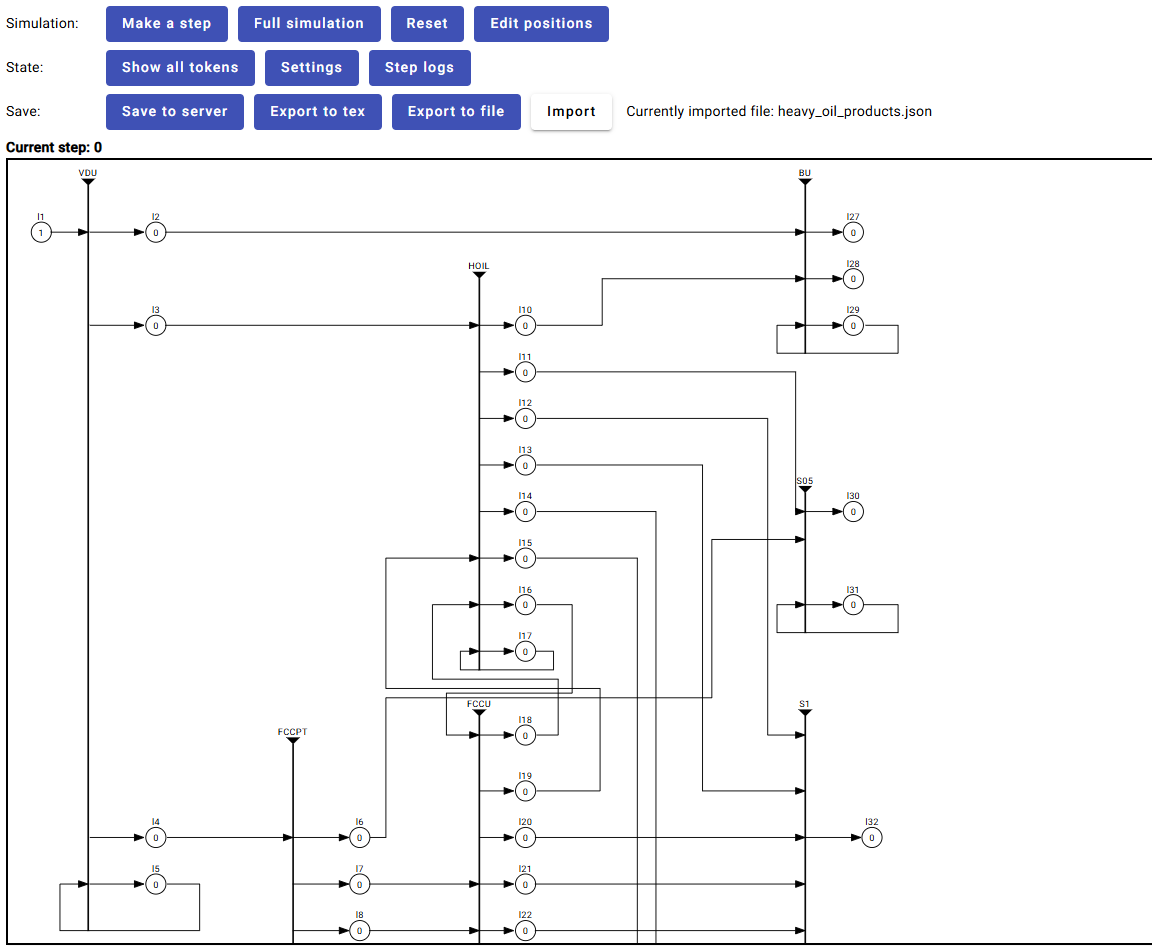
\includegraphics[width=0.95\linewidth]{4. applications/heavyOilProducts/images/model5.png}}
	\captionsetup{width=0.9\textwidth}
	\caption{Модел на обобщена мрежа (ОМ) на веригата за преработка на тежки нефтопродукти в рафинерията.}
	\label{fig:model}
\end{figure}

\paragraph{Начални условия.}
\mbox{}\\
Първоначалното ядро, разположено в позиция $l_1$, представлява атмосферен остатък с характеристична стойност 442.81 (в единици, съответстващи на оригиналния набор данни на рафинерията). Това начално условие е директно зададено в симулацията, както е показано на \textbf{Фигура~\ref{fig:init_token}}.

\begin{figure}[H]
	\centering
	\setlength{\fboxrule}{2pt}
	\setlength{\fboxsep}{0pt}
	\fbox{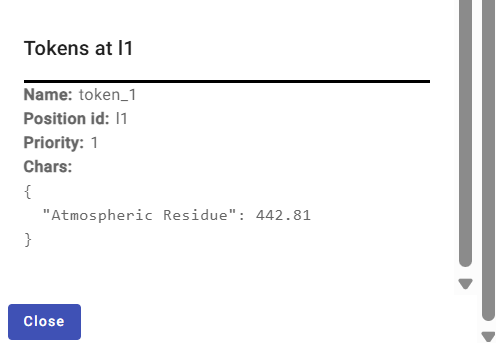
\includegraphics[width=0.6\linewidth]{4. applications/heavyOilProducts/images/init_token_char.png}}
	\captionsetup{width=0.7\textwidth}
	\caption{Инициализация на характеристиката на ядрото за атмосферния остатък в позиция $l_1$.}
	\label{fig:init_token}
\end{figure}

\paragraph{Първи етап на преработка: Вакуумна дестилация.}
\mbox{}\\
В първата моделирана стъпка ядрото за атмосферния остатък (\textit{AR}) се насочва към вакуумната дестилационна инсталация на мазута (\textit{VDU}). Поведението на \textit{VDU} се управлява от нейната индексирана матрица на прехода и съответните характеристични функции. Всяка двойка колона/ред в матрицата определя логиката за насочване на ядрото при зададени условия.

\textbf{Фигура~\ref{fig:vdu_matrix}} представя индексираната матрица за прехода в \textit{VDU}, както е конфигурирана в \textit{OnlineGN}.

\begin{figure}[H]
	\centering
	\setlength{\fboxrule}{2pt}
	\setlength{\fboxsep}{0pt}
	\fbox{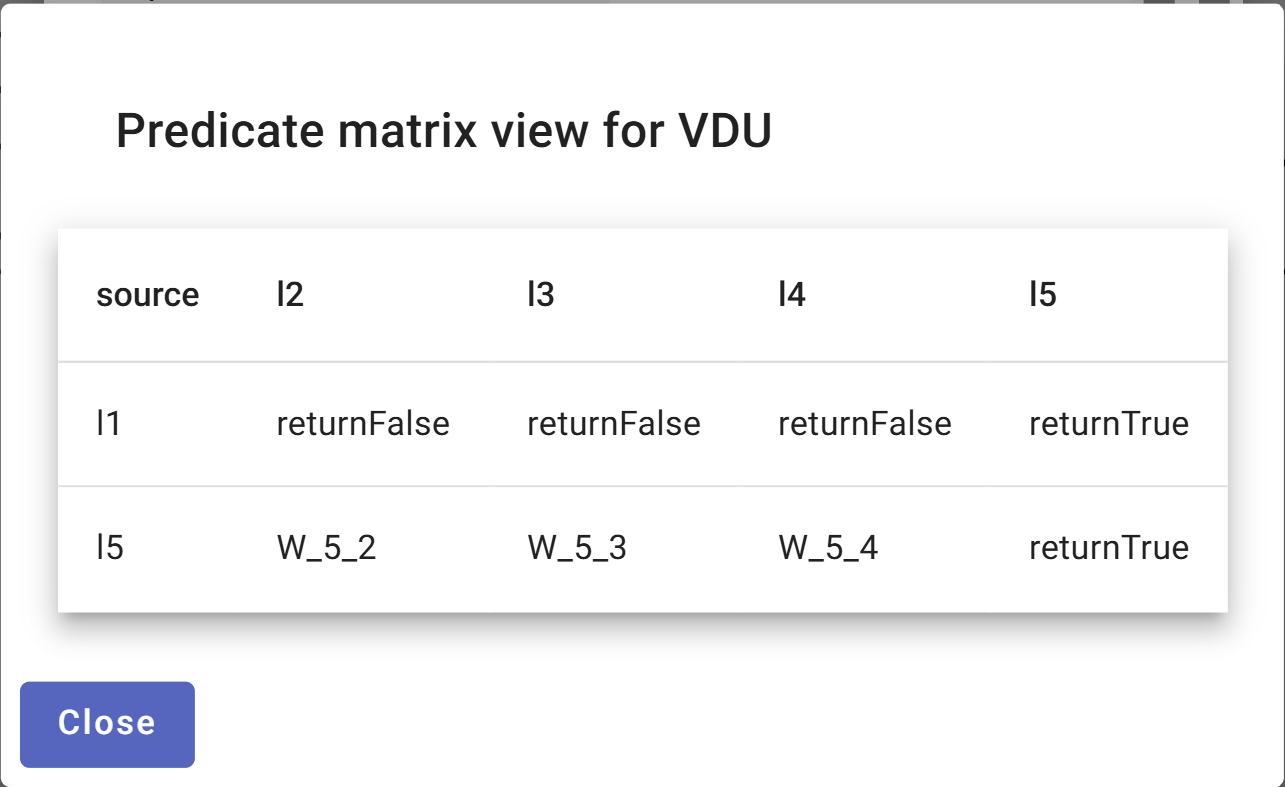
\includegraphics[width=0.6\linewidth]{4. applications/heavyOilProducts/images/matrix1.png}}
	\captionsetup{width=0.7\textwidth}
	\caption{Индексирана матрица на прехода във \textit{VDU}.}
	\label{fig:vdu_matrix}
\end{figure}

За текущия сценарий на симулация се приемат активни заявки от инсталациите \textit{BU}, \textit{H-Oil} и \textit{FCCPT}. Съответно, характеристичните функции („\textit{code}“), свързани с прехода във \textit{VDU}, са зададени както е показано на \textbf{Фигура~\ref{fig:vdu_functions}}. Тези функции могат лесно да бъдат модифицирани, за да отразят промени в потребностите на следващите звена по веригата или в оперативните ограничения.

\begin{figure}[H]
	\centering
	\setlength{\fboxrule}{2pt}
	\setlength{\fboxsep}{0pt}
	\fbox{
\includegraphics[width=0.8\linewidth]{4. applications/heavyOilProducts/images/functions1.png}}
	\captionsetup{width=0.8\textwidth}
	\caption{Характеристични функции, които управляват насочването на ядрото от \textit{VDU} при разглеждания сценарий за търсене.}
	\label{fig:vdu_functions}
\end{figure}

\paragraph{Следващи преработвателни инсталации.}
\mbox{}\\
Същият подход на моделиране се прилага и за останалите технологични звена. Като пример, индексираната матрица на \textit{FCCPT} е показана на \textbf{Фигура~\ref{fig:fccpt_matrix}}. Всяка матрица определя допустимите потоци и логическите условия, при които ядрата извършват преходи между позиции.

\begin{figure}[H]
	\centering
	\setlength{\fboxrule}{2pt}
	\setlength{\fboxsep}{0pt}
	\fbox{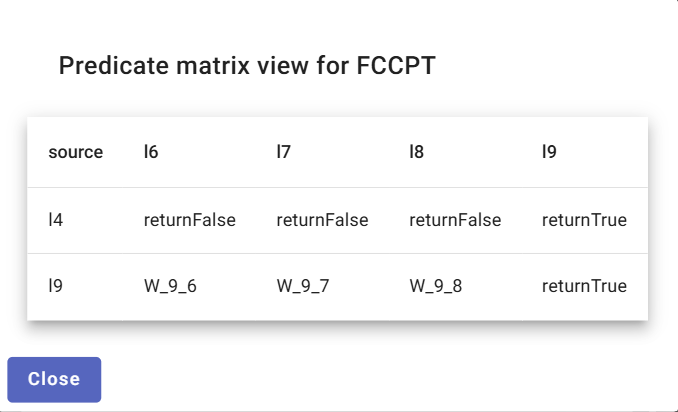
\includegraphics[width=0.6\linewidth]{4. applications/heavyOilProducts/images/matrix2.png}}
	\caption{Индексирана матрица на прехода във \textit{FCCPT}.}
	\label{fig:fccpt_matrix}
\end{figure}

\paragraph{Резултати от симулацията.}
\mbox{}\\
След изпълнение на симулацията на ОМ, количествените резултати за всеки краен продуктов поток се извеждат от характеристиките на ядрата, разположени в съответните позиции. Например количеството мазут с максимално съдържание на сяра до 1.0 мас.\% се определя от характеристичната стойност на ядрото, намиращо се в позиция \(l_{32}\) (\textbf{Фигура~\ref{fig:res1}}).

\begin{figure}[H]
	\centering
	\setlength{\fboxrule}{2pt}
	\setlength{\fboxsep}{0pt}
	\fbox{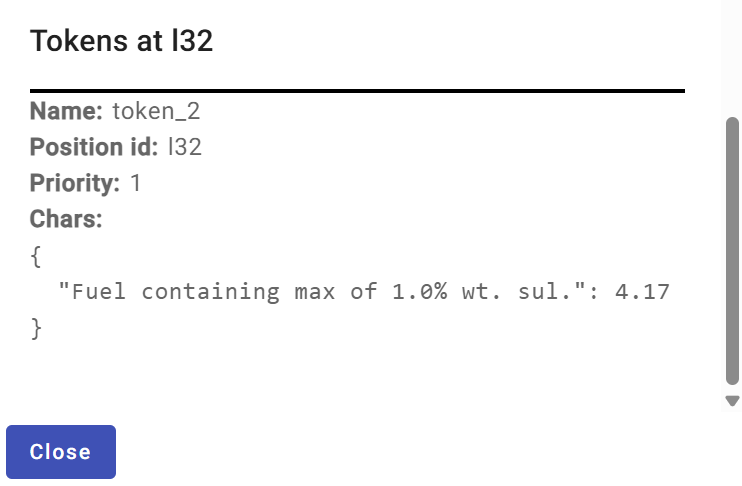
\includegraphics[width=0.6\linewidth]{4. applications/heavyOilProducts/images/1r.png}}
	\captionsetup{width=0.7\textwidth}
	\caption{Полученото количество за мазут с максимум 1.0 мас.\% сяра (позиция $l_{32}$).}
	\label{fig:res1}
\end{figure}

По аналогичен начин, количеството мазут с максимум 2.5 мас.\% сяра се представя от характеристичната стойност на ядрото в позиция $l_{34}$ (\textbf{Фигура~\ref{fig:res2}}).

\begin{figure}[H]
	\centering
	\setlength{\fboxrule}{2pt}
	\setlength{\fboxsep}{1pt}
	\fbox{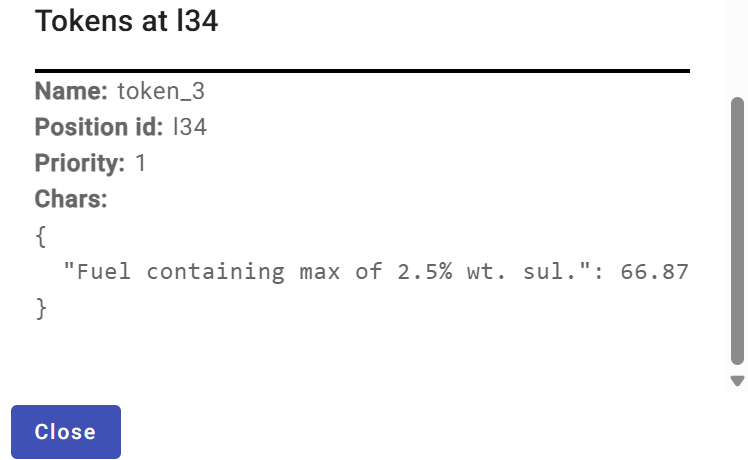
\includegraphics[width=0.6\linewidth]{4. applications/heavyOilProducts/images/2.5r.png}}
	\captionsetup{width=0.7\textwidth}
	\caption{Полученото количество за мазут с максимум 2.5 мас.\% сяра (позиция $l_{34}$).}
	\label{fig:res2}
\end{figure}

\subsubsection{Резултати за модела}

\hspace*{2.5em}Както се вижда на \textbf{Фигура~\ref{fig1}}, производството на трите класа тежко гориво (мазут) и трите класа пътен битум представлява сложен паралелен процес, който включва пет технологични инсталации (\textit{VDU}, \textit{FCCPT}, \textit{FCCU}, \textit{H-Oil} и \textit{BU}), в рамките на които се получават десет рафинирани тежки нефтени продукта. Чрез подходящо смесване на тези десет продукта, отчитащо вариациите в техните физикохимични свойства, разгледани в предходни изследвания~\cite{124}, се получават петте крайни тежки продукта. Този сложен паралелен процес може да бъде моделиран чрез използване на ОМ.

Разработеният ОМ модел за производството на различни класове тежки мазути и пътни битуми в рафинерията е четвъртият и последен модел, след предходните модели за производство на автомобилен бензин~\cite{93}, дизелово гориво~\cite{88}, както и горивен газ, втечнен петролен газ (ВПГ; \textit{LPG}), пропилен и полипропилен~\cite{Stratiev2023_1}.

Представеният модел има обобщен характер и ще бъде част (подмрежа) от бъдещ йерархичен производствен модел. Този ОМ модел от по-високо ниво ще обединява вече разработените модели за производство на отделни рафинирани продукти в едно цяло, което ще позволи цялостен анализ на работата на рафинерията и вземане на решения по отношение на влиянието на различни фактори, като прекъсвания в доставките на суровина, възникване на непланирани спирания, оптимизация на производствения процес, оценка на приложимостта на включването на нови технологични звена и др.

Обикновено линейното програмиране се използва в ситуации, при които е известно, че определено количество суровина с определени характеристики ще бъде доставено след определен период от време. Когато обаче тази яснота липсва поради динамичния характер на процесите, инструментите на линейното програмиране не са достатъчни за адекватно програмиране и планиране -- например при внезапни промени в цената на суровия нефт, в търсенето и предлагането на определени нефтени продукти и др. В рамките на ОМ модел може да се представи всичко, което се получава чрез линейно програмиране, като необходимата информация се задава чрез характеристиките на определени ядра в мрежата.

От друга страна, даден ОМ модел може да бъде включен като подмрежа в ОМ модел на експертна система, вземаща решения за определени ситуации ~\cite{GN-IFS}. Освен това в друга подмрежа могат да се симулират различни сценарии за разглеждания модел с цел проследяване как реален процес би протекъл при конкретни условия. Всеки такъв ОМ ще бъде йерархично включен в следващ модел, който се планира да бъде разработен в близко бъдеще.


\subsubsection{Изводи}

\hspace*{2.5em}Получените резултати показват, че процесите по производство на различни класове тежки нефтени продукти в рафинерия могат да бъдат успешно моделирани чрез ОМ. Подобно на разгледаните в предходната глава производствени вериги, и тук процесите са сложни и паралелни, като ОМ моделът позволява естествено представяне на причинно--следствените зависимости и технологичните ограничения.

Проведената симулация чрез \textbf{\textit{OnlineGN}} води до резултати, съответстващи на очакваното поведение на системата, което служи като верификация на коректността на модела и потвърждава приложимостта на ОМ при моделиране и симулация на производствени процеси в нефтопреработвателна рафинерия.
